\documentclass[a4paper,francais]{article}
\usepackage[T1]{fontenc}
\usepackage[utf8]{inputenc}
\usepackage{amssymb}
\usepackage{braket}
\usepackage{eurosym}
\usepackage{tikz}
\usetikzlibrary{shapes,arrows}
\usepackage{graphicx}
\begin{document}
  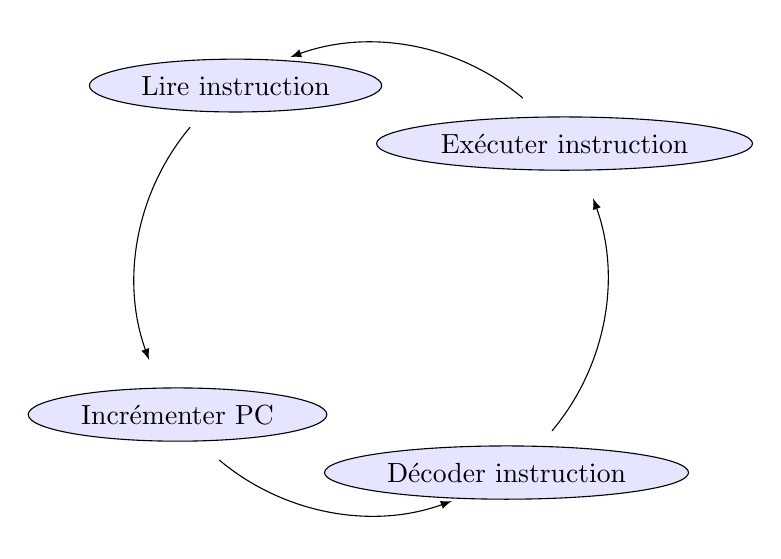
\begin{tikzpicture}
    
\def \angleinit {125}
\def \rayon {3cm}
\def \marge {15}
%\draw[->, >=latex] (125:3) arc (125:215:3);

\tikzstyle{etape} = [draw, ellipse, fill=blue!10]

\node[etape] at (\angleinit:\rayon) {Lire instruction};
\node[etape] at ({\angleinit + 90}:\rayon) {Incrémenter PC};
\node[etape] at ({\angleinit + 180}:\rayon) {Décoder instruction};
\node[etape] at ({\angleinit + 270}:\rayon) {Exécuter
  instruction};
\foreach \s in {0,...,3}
{
  \draw[->, >=latex] ({\angleinit + \s * 90 + \marge}:\rayon)
    arc ({\angleinit + \s * 90 - 360 + \marge}:{\angleinit + ((\s + 1) *
      90 - 360 - \marge)}:\rayon);
}
  \end{tikzpicture}
\end{document}
